\documentclass[12pt, a4paper]{article}
\usepackage{graphicx}
\usepackage{subcaption}
\graphicspath{{images/}}
\title{\LaTeX \space Playground (Local)}
\author{Amritpal Singh\thanks{Learning from the overleaf tutorial}}
\date{3 March 2023}
\begin{document}
\maketitle
	First document in \LaTeX, let's see how it goes lmao.
	I'm typin a few lines to see what happens.
	
	This is another line.
	% deez nuts on a comment tho
	
	This is another another line, hopefully the third. I will
	                        put extra spaces in the actual doc
	          to see how it is rendered
	A complete sentence is on a \textbf{separate} line,
	or \textit{is it}? We're still \emph{continuing} the same 
	\underline{old paragraph}.
	\begin{figure}[h]
		\centering
		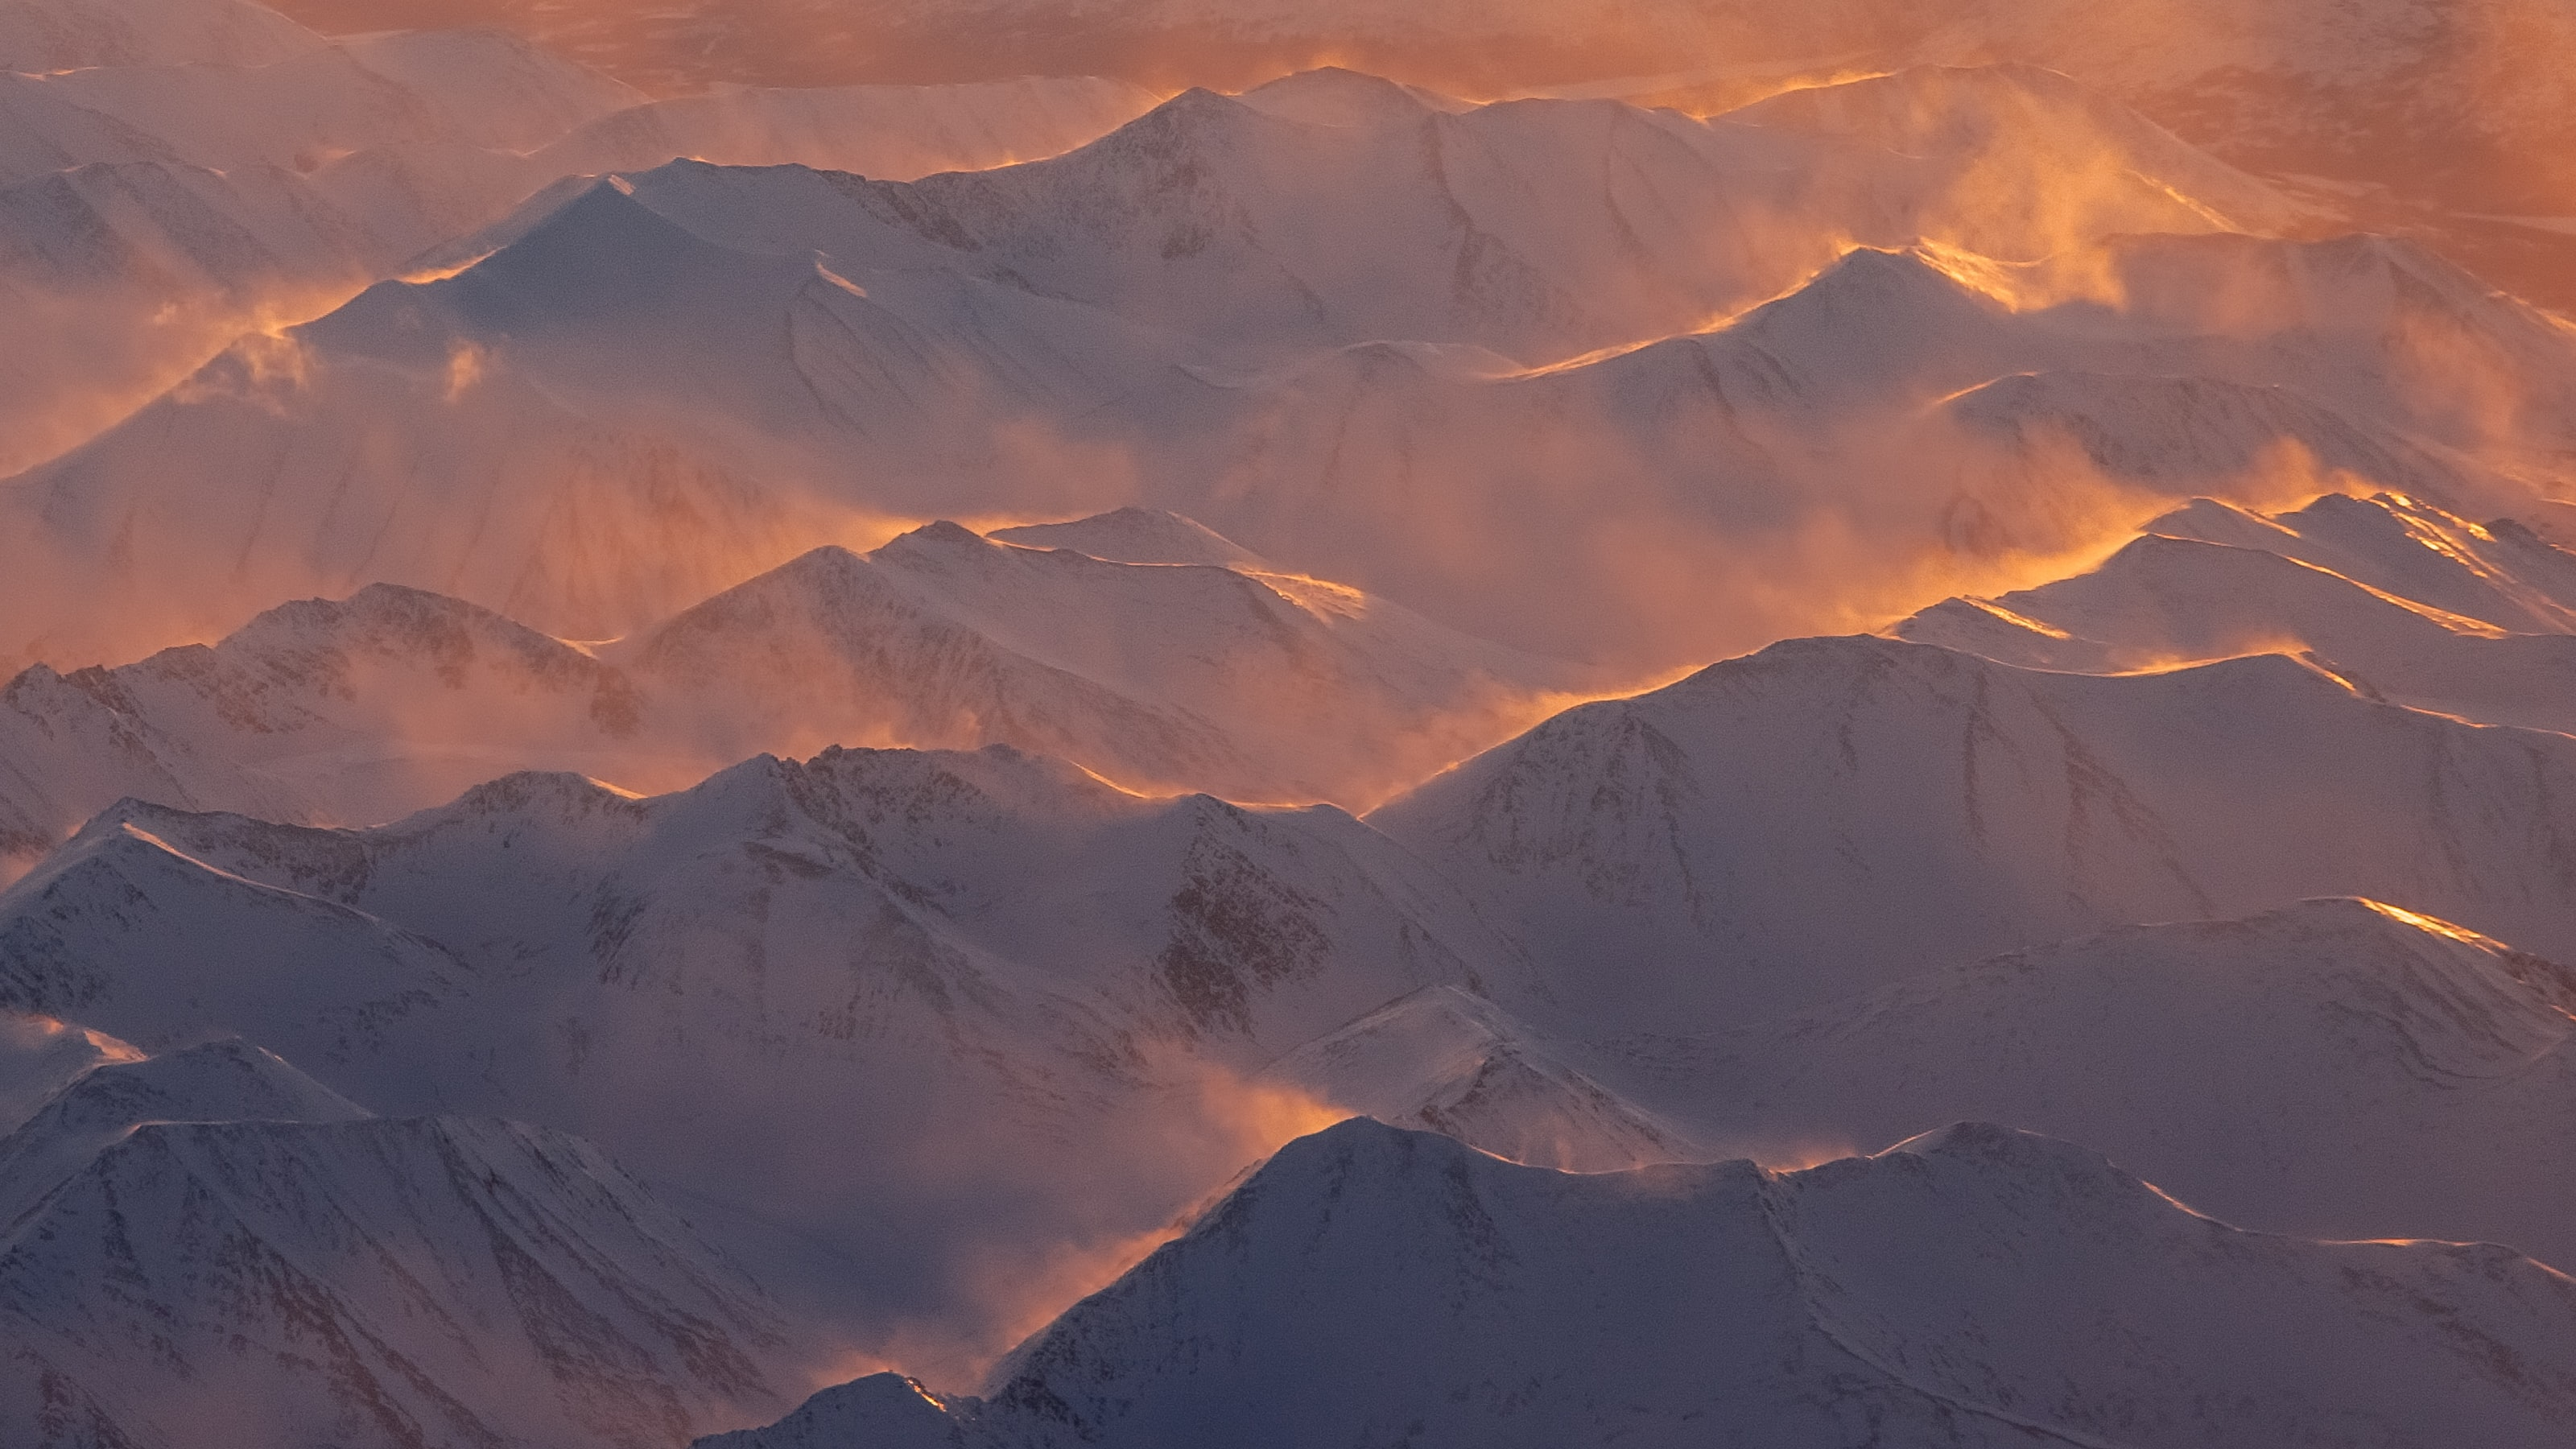
\includegraphics[width=0.75\textwidth,height=0.25\textheight]{windy}
		\caption{A nice orange mountain range}
		\label{fig:mountains1}
	\end{figure}

	The mountain range is really nice to observe while relaxing
	at home. It is a nice orange-ish view where it is rather windy
	it seems.
	
	Now that we've discussed the picture, let us take a look at
	what we have in the store further.
	
	There are two pictures that will be presented on the next page.
	But before we do that, let's see how long I can stretch this text,
	without it having go to the other page. Right now I seem to be doing 
	rather well but I don't know when I will run out of words. Currently,
	It seems that I have run out words but the page as not been turned over,
	or should I rather say, the text has not wrapped to the next page.
	However, it is only for so long that the page can hold my powers before
	I ascend to the next page.
	
	\begin{figure}[h]
		\begin{subfigure}{0.5\textwidth}
			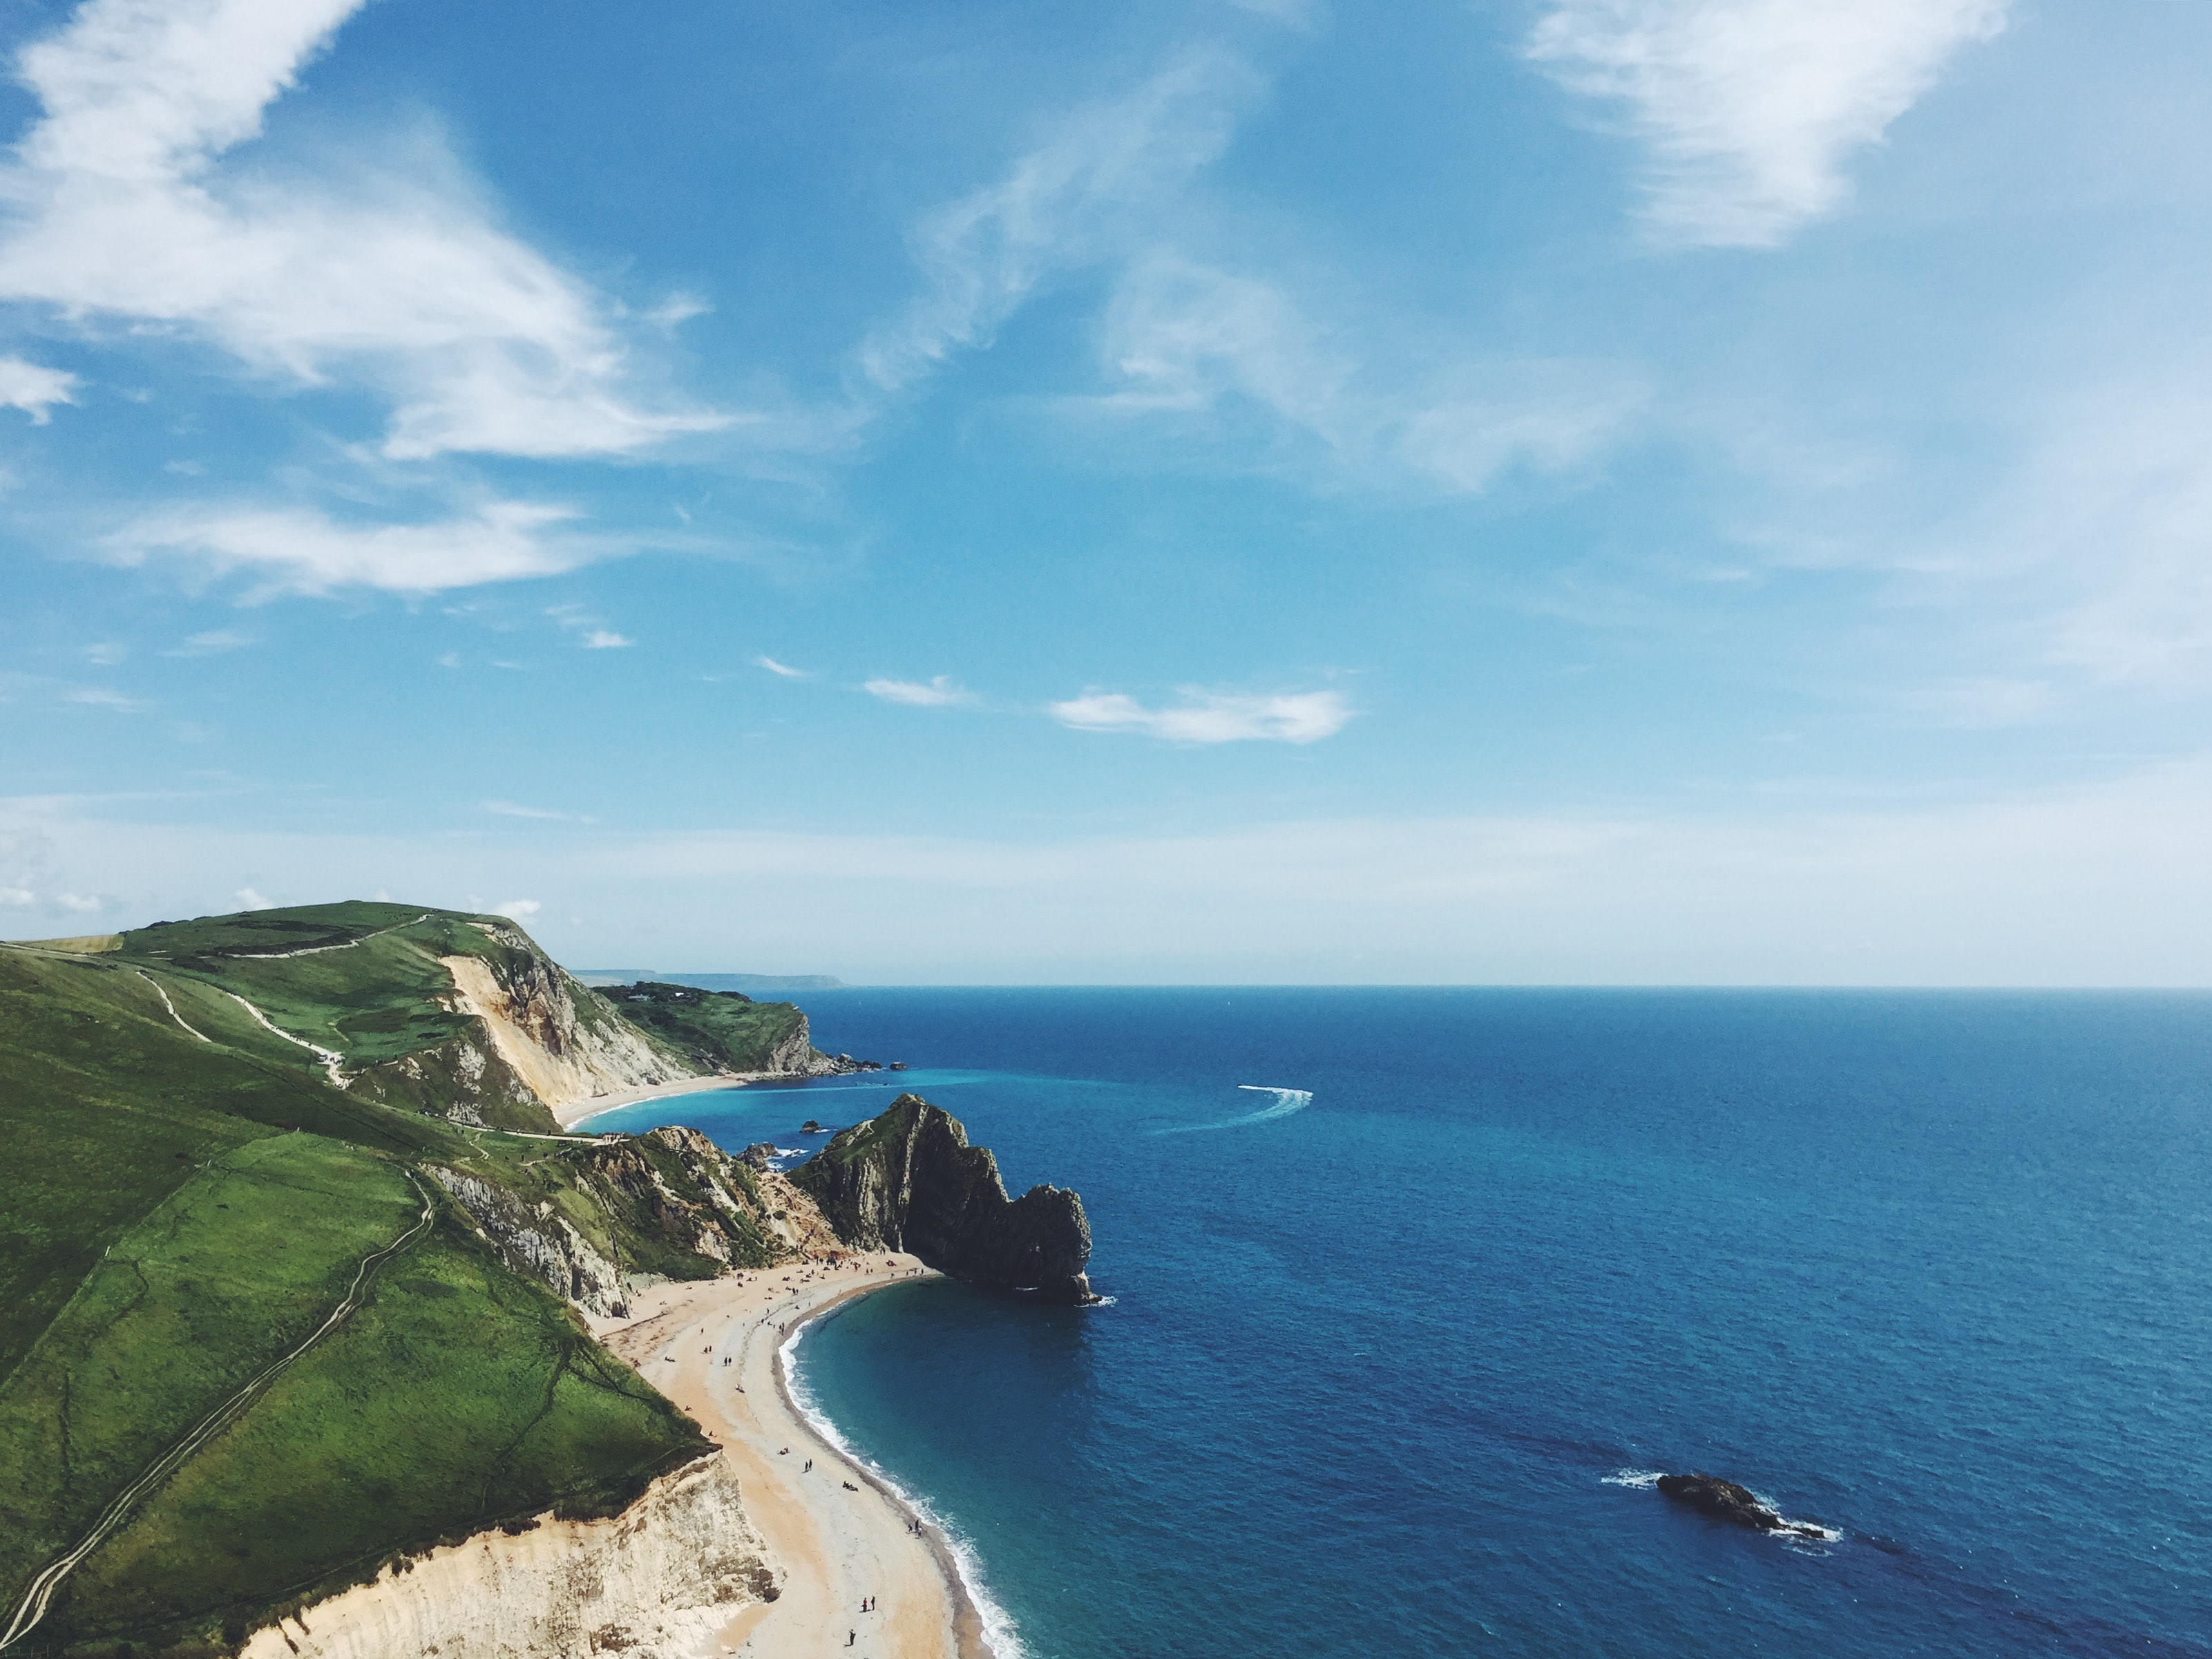
\includegraphics[width=0.9\linewidth, height=6cm]{beach}
			\caption{Beautiful Beach}
			\label{fig:beach1}
		\end{subfigure}
		\begin{subfigure}{0.5\textwidth}
			
\includegraphics[width=0.9\linewidth, height=6cm]{girl}
			\caption{Anime Girl}
			\label{fig:girl1}
		\end{subfigure}
		
		\caption{Two different pictures}
		\label{fig:twoimg}
	\end{figure}
	
	Now that we're done working with photos, let us try and refer to all of them
	here and now. The first picture that we inserted is figure \ref{fig:mountains1}.
	It is a beautiful picture as highlighted before. The third picture comparatively,
	is of a fake Anime Girl (see figure \ref{fig:girl1}). And finally, we have a
	beautiful beach at figure \ref{fig:beach1} where both of these are combined in a
	figure group as figure \ref{fig:twoimg}.
	
\end{document}